\documentclass{report}
\usepackage[utf8]{inputenc}
\usepackage[T1]{fontenc}
\usepackage[brazil]{babel}
\usepackage{graphicx}
\usepackage{amsfonts}
\usepackage{amssymb}
\usepackage{amsmath}
\usepackage{multicol}
\usepackage{ifthen}
\newboolean{firstanswerofthechapter}  
\usepackage{xcolor}
\colorlet{lightcyan}{cyan!40!white}
\usepackage{chngcntr}
\usepackage{stackengine}
\usepackage{tasks}
\usepackage{multirow}
\usepackage{stackengine}
\def\stacktype{L}
\setstackgap{L}{.7\normalbaselineskip}
\stackMath
\usepackage{float}
\newlength{\longestlabel}
\settowidth{\longestlabel}{\bfseries viii.}
%\settasks{counter-format={tsk[r].}, label-format={\bfseries}, label-width=\longestlabel,
    %item-indent=0pt, label-offset=2pt, column-sep={10pt}}
		
\setcounter{secnumdepth}{0} \setlength{\topmargin}{0cm}
\setlength{\headsep}{-0.3cm} \setlength{\textwidth}{17.5cm}
\setlength{\textheight}{23cm} \setlength{\oddsidemargin}{-0.8cm}
\setlength{\evensidemargin}{0cm} \setlength{\footskip}{-1.5cm}

\newcommand{\ad}{{\rm ad}}               %  adjunto
\newcommand{\tr}{{\rm tr}\,}             %  trace
\renewcommand{\dim}{{\rm dim}}           %  dimension
\newcommand{\real}{I\!\!R}               %  real numbers
\renewcommand{\zeta}{Z\! \! \! Z}        %  integer numbers
\newcommand{\ene}{I\! \! N}              %  natural numbers
\newcommand{\rac}{I\! \! \! Q}           %  rational numbers
\newcommand{\com}{\mathbb{C}}            %  complex numbers
\newcommand{\id}{{\rm Id}}               %  aplicaci\'on identidad
\newcommand{\Id}{{\rm Id}}               %  aplicaci\'on identidad
\newcommand{\di}{{\rm dim}}              %  dimensi\'on
\newcommand{\ce}{[\! [}                  %  claudator formes esquerra
\newcommand{\cd}{]\! ]}                  %  claudator formes dreta
\newcommand{\enmor}{{\rm End}\,}         %  Endomorfismes graduats
\newcommand{\Diff}{{\rm Diff}}           %  Op Difer graduats
\newcommand{\Hom}{{\rm Hom}\,}           %  Homomorfismes graduats
\newcommand{\Aut}{{\rm Aut}}             %  Automorfismes graduats

		
\usepackage[lastexercise,answerdelayed]{exercise}
%\counterwithin{Exercise}{chapter}
%\counterwithin{Answer}{chapter}
%\renewcounter{Exercise}[chapter]
%\newcommand{\QuestionNB}{\bfseries\arabic{Question}.\ }
%\renewcommand{\ExerciseName}{Exercício}
%\renewcommand{\ExerciseHeader}{\noindent\def\stackalignment{l}% code from https://tex.stackexchange.com/a/195118/101651
    %\stackunder[0pt]{\colorbox{cyan}{\textcolor{white}{\textbf{\LARGE\ExerciseHeaderNB\;\large\ExerciseName}}}}{\textcolor{lightcyan}{\rule{\linewidth}{2pt}}}\medskip}
\renewcommand{\ExerciseName}{Exercícios}
\renewcommand{\ExerciseHeader}{\noindent\def\stackalignment{l}% code from https://tex.stackexchange.com/a/195118/101651
    \stackunder[0pt]{\colorbox{cyan}{\textcolor{white}{\textbf{\large\ExerciseName}}}}{\textcolor{lightcyan}{\rule{\linewidth}{2pt}}}\medskip}
%\renewcommand{\AnswerName}{Exercises}
%\renewcommand{\AnswerHeader}{\ifthenelse{\boolean{firstanswerofthechapter}}%
    %{\bigskip\noindent\textcolor{cyan}{\textbf{CHAPTER \thechapter}}\newline\newline%
        %\noindent\bfseries\emph{\textcolor{cyan}{\AnswerName\ \ExerciseHeaderNB, page %
                %\pageref{\AnswerRef}}}\smallskip}
    %{\noindent\bfseries\emph{\textcolor{cyan}{\AnswerName\ \ExerciseHeaderNB, page \pageref{\AnswerRef}}}\smallskip}}
%\setlength{\QuestionIndent}{16pt}

\begin{document}

\vspace*{-2cm}

\begin{center}
\begin{minipage}[s]{2cm}
\hspace{-1.3cm}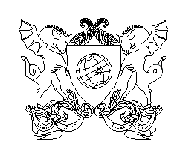
\includegraphics[scale=1.0]{/home/fsbmat/Documentos/GitHub/maf335.github.io/Brasao_UFV/brasaoufv.eps}
\end{minipage}
\begin{minipage}[s]{13cm}
{\begin{center} {\sc \Large Universidade Federal de Vi\c{c}osa}\\
{\sc \large Instituto de Ci\^encias Exatas e Tecnológicas}\\
{\sc \large Campus UFV - Florestal}\\
\end{center}}
\end{minipage}\begin{minipage}[s]{2 cm}
%\includegraphics[width=2 cm]{logoimecc.eps}
\end{minipage}
\end{center}

\vspace{-0.3cm}

%\hline \hline \noindent

%%%%%%%%%%%%%%%%%%%%%%%%%%%%%%%%%%%%%%%%%%%%%%%%%%%%%%%%%%%%%%%%%%%%%%%%%%%

\medskip

\begin{center}

\underline{\underline{{\large{\sc Álgebra Linear A - Gabarito da Lista 2}}}}

\bigskip

{\large {\bf Prof. Fernando Bastos}}
%\bigskip
%
%%{\sc Data: $19/06/2018$}
\end{center}


\begin{enumerate}
\item  (i) $a=-2$ e $b=-9$\qquad (ii) $a=\frac{4}{5}$ e $b=-2$\qquad (iii) $a=-6
$ e $b=8$

(c) $\left| u\right| =5$, $\left\| v\right\| =\sqrt{29}$ e $\left\|
w\right\| =\sqrt{a^{2}+b^{2}}$

\item  $
\begin{array}[t]{llllll}
\text{(i)} & a=7, & b=-3 & \text{e } & c=-2 &  \\
\text{(ii)} & a=9, & b=-6 & \text{e } & c=-12 &  \\
\text{(iii)} & a=5, & b=0 & \text{e} & c=8 &
\end{array}
$

(c)  $\left\| u\right\| =\sqrt{21}$, $\left\| v\right\| =\sqrt{29}$ e $%
\left\| w\right\| =\sqrt{a^{2}+b^{2}+c^{2}}$

\item  $w=(-\frac{\sqrt{10}}{10},-\frac{3\sqrt{10}}{10})$ ou $w=(\frac{\sqrt{%
10}}{10},\frac{3\sqrt{10}}{10})$

\item  Intensidade: $13$ newtons. \ Dire\c{c}\~{a}o: $\theta =\pi
-arctg\left( \frac{5}{12}\right) \;$Sentido: Noroeste

\item  Vetor velocidade $v=(4,-3)$ e $\left\| v\right\| =5$ km/h

\item  $
\begin{array}[t]{ll}
\text{(a)} & U\text{ \'{e} subespa\c{c}o de }V\newline
\\
\text{(b)} & U\text{ n\~{a}o \'{e} subespa\c{c}o de }V\text{\newline
} \\
\text{(c)} & U\text{ n\~{a}o \'{e} subespa\c{c}o de }V\newline
\\
\text{(d)} & U\text{ n\~{a}o \'{e} subespa\c{c}o de }V\newline
\\
\text{(e)} & U\text{ \'{e} subespa\c{c}o de }V\newline
\end{array}
$

\item  (a) L.D. se $k=8$ e L.I. se $k\neq 8$ \newline
(b) L.D. se $k\in \mathbf{R}$

\item  $a-3b-5c=0$

\item  Observe que $\left[ u,v,w,p\right] =\left\{ \left( x,y,z,t\right)
;\;x+3y-7z-7t=0\right\} $\newline
(a) Sim$\qquad \qquad $\ \ \ (b) N\~{a}o\ \ \qquad \qquad \ (c) Sim\ \qquad
\ \qquad \ (d) N\~{a}o

\item  $\left[ S\right] =\left\{ \left[
\begin{array}{rr}
x & y \\
z & t
\end{array}
\right] \in M_{2\times 2}\left( \mathbf{R}\right) ;\ 7x-5y+18z+7t=0\right\} $

\item  (a) ( L.D.) \qquad (b) ( L.D.) \qquad (c) ( L.D.) \qquad (d) ( L.I.) $%
\qquad $(e) ( L.I.)

\item  (a) (V) \qquad (b) ( F) \qquad (c) (V)\qquad (d) ( V) \qquad (e) (F)

\item

\item  $\left\{
\begin{array}{l}
2x+y+z=0 \\
5x+y-t=0
\end{array}
\right. $

\item  L.I.

\item

\item  (b) $\left[
\begin{array}{rr}
0 & \;-2 \\
0 & 1
\end{array}
\right] \in W$ e $\left[
\begin{array}{rr}
0 & \;2 \\
3 & 1
\end{array}
\right] \notin W$\newline
(c) Base: $\left\{ \left[
\begin{array}{rr}
2 & \;1 \\
0 & 1
\end{array}
\right] ,\;\left[
\begin{array}{rr}
0 & \;-2 \\
0 & 1
\end{array}
\right] \right\} $

\item  (b) Base de $\mathbf{W}_{1}:$\newline
$\left\{ \left[
\begin{array}{rrr}
1 & 0 & 0 \\
0 & 0 & 0 \\
0 & 0 & 0
\end{array}
\right] ,\;\left[
\begin{array}{lll}
0 & 1 & 0 \\
1 & 0 & 0 \\
0 & 0 & 0
\end{array}
\right] ,\text{\ }\left[
\begin{array}{lll}
0 & 0 & 1 \\
0 & 0 & 0 \\
1 & 0 & 0
\end{array}
\right] ,\;\left[
\begin{array}{lll}
0 & 0 & 0 \\
0 & 1 & 0 \\
0 & 0 & 0
\end{array}
\right] ,\;\left[
\begin{array}{lll}
0 & 0 & 0 \\
0 & 0 & 1 \\
0 & 1 & 0
\end{array}
\right] ,\;\left[
\begin{array}{lll}
0 & 0 & 0 \\
0 & 0 & 0 \\
0 & 0 & 1
\end{array}
\right] \right\} $

\item  (b) Base de $\mathbf{W}_{2}:$ $\left\{ \left[
\begin{array}{rrr}
0 & \;1 & \;0 \\
-1 & 0 & 0 \\
0 & 0 & 0
\end{array}
\right] ,\text{\ }\left[
\begin{array}{rrr}
0 & 0 & 1 \\
0 & \;0 & \;0 \\
-1 & 0 & 0
\end{array}
\right] ,\;\left[
\begin{array}{rrr}
0 & 0 & 0 \\
0 & 0 & 1 \\
0 & \;-1 & \;0
\end{array}
\right] \right\} $

\item  Observe que para toda matriz $A\in M_{3\times 3}(\mathbf{R})$, temos:

\begin{align*}
A=&\stackunder{\text{Sim\'{e}trica}}{\underbrace{ }}+\stackunder{\text{Anti-sim\'{e}trica}}{\underbrace{ }}\\
=&\frac{1}{2}\left(
A+A^{T}\right) +\frac{1%
}{2}\left( A-A^{T}\right) 
\end{align*}

%$A=\stackunder{\text{Sim\'{e}trica}}{\underbrace{\frac{1}{2}\left(
%A+A^{T}\right) }}+\stackunder{\text{Anti-sim\'{e}trica}}{\underbrace{\frac{1%
%}{2}\left( A-A^{T}\right) }}$.

\item  $\dim D=3$. Uma base para este subespa\c{c}o \'{e}\newline
$\left\{ \left[
\begin{array}{rrr}
1 & 0 & 0 \\
0 & 0 & 0 \\
0 & 0 & 0
\end{array}
\right] ,\;\left[
\begin{array}{lll}
0 & 0 & 0 \\
0 & 1 & 0 \\
0 & 0 & 0
\end{array}
\right] ,\;\left[
\begin{array}{lll}
0 & 0 & 0 \\
0 & 0 & 0 \\
0 & 0 & 1
\end{array}
\right] \right\} $

\item  $\dim D=6$. Uma base para este subespa\c{c}o \'{e}\newline
$\left\{ \left[
\begin{array}{rrr}
1 & 0 & 0 \\
0 & 0 & 0 \\
0 & 0 & 0
\end{array}
\right] ,\;\left[
\begin{array}{lll}
0 & 1 & 0 \\
0 & 0 & 0 \\
0 & 0 & 0
\end{array}
\right] ,\text{\ }\left[
\begin{array}{lll}
0 & 0 & 1 \\
0 & 0 & 0 \\
0 & 0 & 0
\end{array}
\right] ,\;\left[
\begin{array}{lll}
0 & 0 & 0 \\
0 & 1 & 0 \\
0 & 0 & 0
\end{array}
\right] ,\;\left[
\begin{array}{lll}
0 & 0 & 0 \\
0 & 0 & 1 \\
0 & 0 & 0
\end{array}
\right] ,\;\left[
\begin{array}{lll}
0 & 0 & 0 \\
0 & 0 & 0 \\
0 & 0 & 1
\end{array}
\right] \right\} $

\item  (a) $\dim S=2$ e $\mathcal{B}_{S}=\left\{ \left( 11,0,-5,1\right)
,\;\left( -2,1,0,0\right) \right\} $\newline
(b) $\dim S=3$ e $\mathcal{B}_{S}=\left\{ \left( -2,1,0,0,0\right) ,\;\left(
5,0,-2,1,0\right) ,\;\left( -7,0,2,0,1\right) \right\} $

\item  $
\begin{array}[t]{lll}
\text{(a)} & \dim U=2\text{,} & U=\left\{ (x,y,3y-3x,y-2x);\;x,y\in \mathbf{R%
}\right\}  \\
\text{(b)} & \dim W=2\text{,} & W=\left\{ (x,y,2y-2x,-y);\;x,y\in \mathbf{R}%
\right\}  \\
\text{(c)} & \dim (U\cap W)=1\text{,} & U\cap W=\left\{ (x,x,0,-x);\;x\in
\mathbf{R}\right\}  \\
\text{(d)} & \dim (U+W)= & \dim U+\dim W-\dim (U\cap W)=3
\end{array}
$ \qquad  \qquad \qquad

\item  (b) $
\begin{array}[t]{l}
\mathcal{B}_{W_{1}}=\left\{ (1,0,-1,0),(0,1,0,0),(0,0,0,1)\right\}
\smallskip  \\
\mathcal{B}_{W_{2}}=\left\{ (1,0,0,0),(0,1,0,-1),(0,0,1,0)\right\}
\smallskip  \\
\mathcal{B}_{W_{1}\cap W_{2}}=\left\{ (1,0,-1,0),(0,1,0,-1)\right\}
\smallskip
\end{array}
$\newline
(c) $W_{1}+$ $W_{2}=\mathbf{R}^{4}$, pois $\dim (W_{1}+$ $W_{2})=\dim
W_{1}+\dim W_{2}+\dim W_{1}\cap W_{2}=3+3-2=4$.

\item  $
\begin{array}[t]{ll}
\text{(a)} & \mathcal{B}_{W}=\left\{ (1,0,0,-1),(0,1,0,-1),\left(
0,0,1,1\right) \right\} \text{\textit{\ \ }e}\mathit{\ \ }\dim W=3\newline
\\
\text{(b)} & \mathit{\ }u=\left( 2,-3,2,2\right) \notin W\newline
\\
\text{(c)} & x+y-z+t=0
\end{array}
$

\item  $\dim \left[ S\right] =6$, $\dim \left[ R\right] =3$, $\dim \left(
\left[ S\right] \cap \left[ R\right] \right) =3$ e $\dim \left( \left[
S\right] +\left[ R\right] \right) =6$

\item  $
\begin{array}[b]{llllll}
\text{(a) }\left[ I\right] _{\mathcal{C}}^{\mathcal{\gamma }}=\left[
\begin{array}{rrr}
1 & 0 & \;1 \\
0 & 1 & 0 \\
2 & \;-1 & 1
\end{array}
\right]  &  &  &  &  & \text{(b) }\left[ u\right] _{\gamma }=\left[
\begin{array}{l}
1 \\
1 \\
0
\end{array}
\right]
\end{array}
\qquad \qquad $\qquad

\item  $
\begin{array}{llllll}
\text{(b) (i)}\;\left[ v\right] _{\mathcal{B}}=\left[
\begin{array}{l}
0 \\
1 \\
1
\end{array}
\right]  &  & \qquad  & \qquad  &  & \text{(ii) }\left[ w\right] _{\mathcal{B%
}}=\left[
\begin{array}{l}
1 \\
2 \\
0
\end{array}
\right]
\end{array}
\qquad $ \qquad \qquad \qquad \qquad $.$

\item  $\mathcal{B}_{s}=\left\{ x^{3}-3x-2,\;x^{2}-2x-3\right\} $ e $\dim S=2
$.

\item  $_{
\begin{array}[t]{ll}
\dim U=3\text{,} & \mathcal{B}_{U}=\left\{ \left( 1,0,0,0\right) ,\left(
0,1,0,-1\right) ,\left( 0,0,1,-1\right) \right\} \smallskip  \\
\dim W=2\text{,} & \mathcal{B}_{W}=\left\{ \left( 1,-1,0,0\right) ,\left(
0,0,2,1\right) \right\} \smallskip  \\
\dim \left( U\cap W\right) =1\text{,} & \mathcal{B}_{U\cap W}=\left\{ \left(
3,-3,2,1\right) \right\} \smallskip \smallskip  \\
\dim \left( U+W\right) =4\text{,} & \mathcal{B}_{U+W}=\left\{ \left(
1,0,0,0\right) ,\left( 0,1,0,-1\right) ,\left( 0,0,1,-1\right) ,\left(
1,-1,0,0\right) \right\}
\end{array}
}$\newline

\item  $
\begin{array}[t]{ll}
\text{(a) }\left\{
\begin{array}{l}
-3x-4y+z+w=0 \\
4x+2y+t=0
\end{array}
\right. \qquad \text{ e} & \qquad \left\{
\begin{array}{l}
9x+2y+z+w=0 \\
-4x-2y+t=0
\end{array}
\right. \smallskip  \\
\text{(b) }\mathcal{B}_{\mathbf{U}\cap \mathbf{W}}=\left\{ \left(
1,-2,-5,0,0\right) ,\;\left( 0,0,-1,0,1\right) \right\} \text{ e} & \qquad
\dim \left( \mathbf{U}\cap \mathbf{W}\right) =2\smallskip \smallskip  \\
\text{(c) }\dim \left( \mathbf{U}+\mathbf{W}\right) =4 &
\end{array}
\qquad \,$\newline

\item  $\alpha =\left\{ \left( \frac{1}{2},\frac{1}{2},\frac{1}{2}\right)
,\left( \frac{1}{2},-\frac{1}{2},\frac{1}{2}\right) ,\left( \frac{1}{2},-%
\frac{1}{2},-\frac{1}{2}\right) \right\} .$

\item  $
\begin{array}[t]{lllll}
\text{(a) }\left[ v\right] _{\alpha }=\left[
\begin{array}{r}
1 \\
1 \\
-4
\end{array}
\right]  &  &  &  & \text{(b) }\left[ v\right] _{\beta }=\left[
\begin{array}{r}
2 \\
-3 \\
-1
\end{array}
\right]
\end{array}
\qquad $

\item  $
\begin{array}[t]{lllll}
\left[ I\right] _{\beta _{1}}^{\beta _{2}}=\left[
\begin{array}{rr}
\frac{4}{11} & \;-\frac{3}{11} \\
\frac{1}{11} & \frac{2}{11}
\end{array}
\right]  &  & \text{e} &  & \left[ \left( 5,-8\right) \right] _{\beta
_{1}}=\left[
\begin{array}{c}
4 \\
-1
\end{array}
\right]
\end{array}
$

\item  $
\begin{array}[t]{lllll}
\text{(a)} & \text{(i) }\left[ I\right] _{\beta }^{\beta _{1}}=\left[
\begin{array}{rr}
-1 & 1 \\
1 & 1
\end{array}
\right]  & \text{(ii) }\left[ I\right] _{\beta _{1}}^{\beta }=\left[
\begin{array}{rr}
-\frac{1}{2} & \frac{1}{2} \\
\frac{1}{2} & \frac{1}{2}
\end{array}
\right]  & \text{(iii) }\left[ I\right] _{\beta _{2}}^{\beta }=\left[
\begin{array}{rr}
\frac{\sqrt{3}}{6} & \frac{1}{2} \\
\frac{\sqrt{3}}{6} & -\frac{1}{2}
\end{array}
\right]  & \text{(iv) }\left[ I\right] _{\beta _{3}}^{\beta }=\left[
\begin{array}{rr}
\frac{1}{2} & 0 \\
0 & \frac{1}{2}
\end{array}
\right] \smallskip  \\
\text{(b)} & \text{(i) }\left[ v\right] _{\beta }=\left[
\begin{array}{r}
3 \\
-2
\end{array}
\right]  & \text{(ii) }\left[ v\right] _{\beta _{1}}=\left[
\begin{array}{r}
-\frac{5}{2} \\
\frac{1}{2}
\end{array}
\right]  & \text{(iii) }\left[ v\right] _{\beta _{2}}=\left[
\begin{array}{r}
-\frac{2-\sqrt{3}}{2} \\
\frac{2+\sqrt{3}}{2}
\end{array}
\right]  & \text{(iv) }\left[ v\right] _{\beta _{3}}=\left[
\begin{array}{r}
\frac{3}{2} \\
-1
\end{array}
\right] \smallskip  \\
\text{(c)} & \text{(i) }\left[ v\right] _{\beta }=\left[
\begin{array}{r}
-4 \\
4
\end{array}
\right]  & \text{(ii) }\left[ v\right] _{\beta _{2}}=\left[
\begin{array}{r}
\frac{6-2\sqrt{3}}{3} \\
\frac{-6-2\sqrt{3}}{3}
\end{array}
\right]  & \text{(iii) }\left[ v\right] _{\beta _{3}}=\left[
\begin{array}{r}
-2 \\
2
\end{array}
\right]  & \smallskip
\end{array}
$

\item  \ $
\begin{array}[t]{llll}
\text{(a)} & \text{(i) }\left[ I\right] _{\beta _{1}}^{\beta _{2}}=\left[
\begin{array}{rr}
-1 & 1 \\
0 & \frac{1}{2}
\end{array}
\right]  & \text{(ii) }\left[ I\right] _{\beta _{2}}^{\beta _{3}}=\left[
\begin{array}{rr}
0 & -1 \\
-1 & -1
\end{array}
\right]  & \text{(iii) }\left[ I\right] _{\beta _{1}}^{\beta _{3}}=\left[
\begin{array}{rr}
-1 & 0 \\
-\frac{1}{2} & -\frac{1}{2}
\end{array}
\right]  \\
& \text{(iv) }\left[ I\right] _{\beta _{1}}^{\beta _{2}}\left[ I\right]
_{\beta _{2}}^{\beta _{3}}=\left[
\begin{array}{rr}
-1 & 0 \\
-\frac{1}{2} & -\frac{1}{2}
\end{array}
\right]  &  &  \\
\text{(b)} & \left[ I\right] _{\beta _{1}}^{\beta _{3}}=\left[ I\right]
_{\beta _{1}}^{\beta _{2}}\left[ I\right] _{\beta _{2}}^{\beta _{3}} &  &
\end{array}
$ $\;\;\;\;\;\;\;$\newline
\qquad \newline
\end{enumerate}

\end{document}